\documentclass[a4paper]{scrartcl}

\usepackage{float}
\usepackage{tikz}
\usetikzlibrary{arrows,automata}
\usepackage{pgf}
\usepackage[utf8]{inputenc} % this is needed for umlauts
\usepackage[ngerman]{babel} % this is needed for umlauts
\usepackage[T1]{fontenc}    % this is needed for correct output of umlauts in pd
\usepackage{amssymb}
\usepackage{amsmath}
\usepackage{mathrsfs}
\usepackage{dsfont}
\usepackage{graphicx}
\usepackage{fancyhdr}
\usepackage{lastpage}
\usepackage{imakeidx}
\setlength{\parskip}{\medskipamount}
\setlength{\parindent}{0pt}
\usepackage{enumitem}
\usepackage{hyperref}

%%%%%%%%%%%%%%%%%%%%%%%%
% Kopf- und Fusszeilen %
%%%%%%%%%%%%%%%%%%%%%%%%
\pagestyle{fancy}
\lhead{
        Maximilian Roth
}
\chead{Logik-Tutorat Lösungen Blatt 3\\}
\rhead{
        \today{} \\
        Seite \thepage{} von \pageref{LastPage}\\
        
}
\lfoot{}
\cfoot{}
\rfoot{} 

%%%%%%%%%%%%%%%%%%%%%%%%
% Anfang des Dokuments %
%%%%%%%%%%%%%%%%%%%%%%%%

\begin{document}
\section*{Disclaimer}%
\label{sec:disclaimer}
Auch in diesem Dokument können sich Fehler befinden!\\
Sie sind nicht die Musterlösung der Aufgaben, sondern selbst erstellte Lösungen.\\

Als generelle Lektüre kann ich nur das Skript von Markus Junker aus dem WS 17/18 empfehlen:\\
\url{http://home.mathematik.uni-freiburg.de/junker/skripte/InfoLogik.pdf}\\
Hier ist vieles sehr genau und verständlich erklärt.

\section*{}%
\label{sec:aufgabe_1}
    \begin{figure}[H]
        \centering
        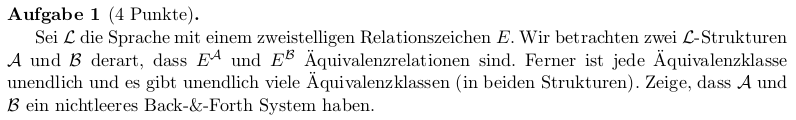
\includegraphics[scale=0.6]{./A-1.png}
        \label{fig:}
    \end{figure} 



\section*{}%
\label{sec:aufgabe_2}

    \begin{figure}[H]
        \centering
        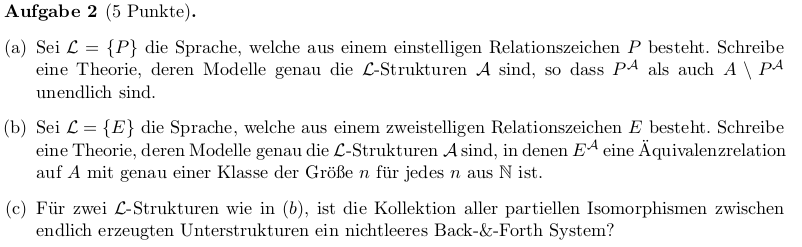
\includegraphics[scale=0.6]{./A-2.png}
        \label{fig:}
    \end{figure}

    Eine Theorie ist eine Menge T von $\mathscr{L}$-Aussagen.

    \begin{itemize}
        \item a)\\
            $T = A_1 \cup A_2$\\
            $A_1 = \{\exists x_1 \dots \exists x_n (\bigwedge_{i \neq j}(\neg x_i \doteq x_j \land P(x_i,x_j))) | n \in \mathds{N}\}$\\
            Also keine zwei Variablen sind gleich und alle n sind in Relation\\
            $\Rightarrow$ Es gibt min n Elemente in P $\forall n \in \mathds{N}$\\
            $\Rightarrow$ Es gibt unendlich viele Elemente in P\\
            \\$A_2 = \{\exists x_1 \dots \exists x_n (\bigwedge_{i \neq j}(\neg x_i \doteq x_j \land \neg P(x_i,x_j))) | n \in \mathds{N}\}$\\
            Es sind also mindestens n Elemente nicht in P $\forall n \in \mathds{N}$\\
            $\Rightarrow$ Es gibt unendlich viele Elemente, die nicht in P liegen.\\
            \\Aus $T = A_1 \cup A_2$ folgt, dass unendlich viele Elemente in P sind und unendlich viele es nicht sind.\\

        \item b)\\

    \end{itemize}


\section*{}%
\label{sec:aufgabe_3}

    \begin{figure}[H]
        \centering
        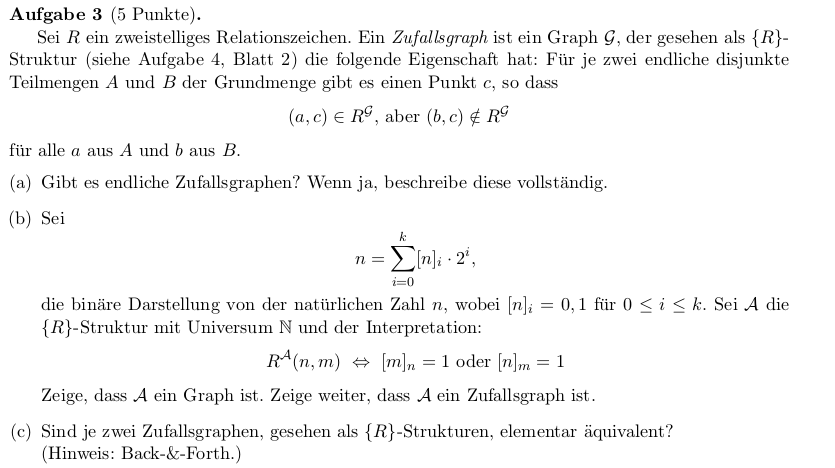
\includegraphics[scale=0.6]{./A-3.png}
        \label{fig:}
    \end{figure}

\section*{}%
\label{sec:aufgabe_4}

    \begin{figure}[H]
        \centering
        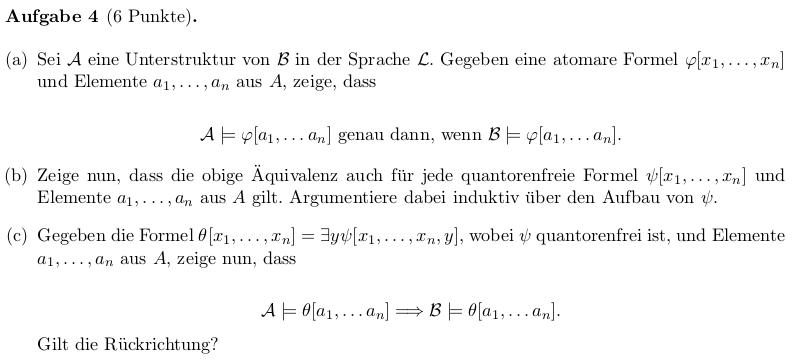
\includegraphics[scale=0.6]{./A-4.png}
        \label{fig:}
    \end{figure}

\end{document}

